\documentclass[10pt]{article}

%Math
\usepackage{amsmath}
\usepackage{amsfonts}
\usepackage{amssymb}
\usepackage{amsthm}
\usepackage{ulem}
\usepackage{stmaryrd} %f\UTF{00FC}r Blitz!
\usepackage{tikz}

%PageStyle
\usepackage[ngerman]{babel} % deutsche Silbentrennung
\usepackage[utf8]{inputenc} 
\usepackage{fancyhdr, graphicx}
\usepackage[scaled=0.92]{helvet}
\usepackage{enumitem}
\usepackage{parskip}
\usepackage[a4paper,top=2cm]{geometry}
\setlength{\textwidth}{17cm}
\setlength{\oddsidemargin}{-0.5cm}


%My Commands
\newcommand{\RN}{\mathbb{R}} %Real Number
\newcommand{\NN}{\mathbb{N}} %Natural Number
\newcommand{\QN}{\mathbb{Q}} %Rational Number
\newcommand{\ZN}{\mathbb{Z}} %ganze Zahlen
\newcommand{\CN}{\mathbb{C}}
\newcommand{\Teilt}{\mid} %|
\newcommand{\Teiltn}{\nmid} %kein teiler
\newcommand{\Potp}{\mathcal{P}} %Potenzmenge
\newcommand{\Pota}{\mathcal{A}}
\newcommand{\Potr}{\mathcal{R}}
\newcommand{\Potn}{\mathcal{N}}
\newcommand{\Bold}[1]{\textbf{#1}} %Boldface
\newcommand{\Kursiv}[1]{\textit{#1}} %Italic
\newcommand{\T}[1]{\text{#1}} %Textmode
\newcommand{\Nicht}[1]{\T{\sout{$ #1 $}}} %Streicht Shit durch
\newcommand{\lra}{\leftrightarrow} %Arrows
\newcommand{\ra}{\rightarrow}
\newcommand{\la}{\leftarrow}
\newcommand{\lral}{\longleftrightarrow}
\newcommand{\ral}{\longrightarrow}
\newcommand{\lal}{\longleftarrow}
\newcommand{\Lra}{\Leftrightarrow}
\newcommand{\Ra}{\Rightarrow}
\newcommand{\La}{\Leftarrow}
\newcommand{\Lral}{\Longleftrightarrow}
\newcommand{\Ral}{\Longrightarrow}
\newcommand{\Lal}{\Longleftarrow}
\newcommand{\Vektor}[1]{\vec{#1}}
\newcommand{\Brace}[1]{\left( #1 \right)} %()
\newcommand{\Bracel}[1]{\left\lbrace #1 \right.} %(
\newcommand{\Bracer}[1]{\right. #1 \right\rbrace} %)
\newcommand{\Brack}[1]{\left\lbrace #1 \right\rbrace} %{}
\newcommand{\Brackl}[1]{\left\lbrace #1 \right.} %{
\newcommand{\Brackr}[1]{\right. #1 \right\rbrace} %}
\newcommand{\Result}[1]{\underline{\underline{#1}}} %Doppelt unterstrichen
\newcommand{\Abs}[1]{\left| #1 \right|} %Absolutbetrag
\newcommand{\Norm}[1]{\Abs{\Abs{ #1 }}} %Norm
\newcommand{\Arrays}[1]{\left(\begin{array}{c}#1\end{array}\right)} %Array mit einer Kolonne ()
\newcommand{\Array}[2]{\left(\begin{array}{#1}#2\end{array}\right)} %Array mit n Kolonnen ()
\newcommand{\Bracka}[2]{\left\lbrace\begin{array}{#1}#2\end{array}\right\rbrace} %Array mit {}
\newcommand{\Brackal}[2]{\left\lbrace\begin{array}{#1} #2 \end{array}\right.} %Array mit {
\newcommand{\Brackar}[2]{\left.\begin{array}{#1} #2 \end{array}\right\rbrace} %Array mit }
\newcommand{\Sumone}[2]{\sum_{#2=1}^{#1}} %Summe von 1
\newcommand{\Sumz}[2]{\sum_{#2=0}^{#1}} %Summe von 0
\newcommand{\Sum}[2]{\sum_{#2}^{#1}} %Allgemeine Summe
\newcommand{\Oneover}[1]{\frac{1}{#1}} %1 über igendwas
\newcommand{\Tablewt}[3]{\begin{table*}[h]\caption{#1} \begin{tabular}{#2}{#3}\end{tabular}\end{table*}} %Table mit Titel
\newcommand{\Oben}[2]{\overset{#1}{#2}} %etwas über etwas anderem
\newcommand{\Unten}[2]{\underset{#1}{#2}} %etwas unter etwas anderem
\newcommand{\Bildcap}[2]{\begin{figure}[htb]\centering\includegraphics[width=0.2\textwidth]{#1} \caption{#2}\end{figure}} %Bild mit beschriftung
\newcommand{\Bildjpeg}[1]{\includegraphics[width=0.2\textwidth]{#1.jpeg}} %Bilder jpeg!!
\newcommand{\Bildjpg}[1]{\includegraphics[width=0.2\textwidth]{#1.jpg}} %Bilder jpg!!
\newcommand{\Bild}[1]{\includegraphics[width=0.4\textwidth]{#1}} %Bilder jpg!!
%Beispiel für lstlisting \lstinputlisting[label=Aufgabe 4a,caption=Aufgabe 4a]{4a.java}

% Code listenings
\usepackage{color}
\usepackage{xcolor}
\usepackage{listings}
\usepackage{caption}
\DeclareCaptionFont{white}{\color{white}}
\DeclareCaptionFormat{listing}{\colorbox{gray}{\parbox{\textwidth}{#1#2#3}}}
\captionsetup[lstlisting]{format=listing,labelfont=white,textfont=white}
\lstdefinestyle{JavaStyle}{
 language=Java,
 basicstyle=\footnotesize\ttfamily, % Standardschrift
 numbers=left,               % Ort der Zeilennummern
 numberstyle=\tiny,          % Stil der Zeilennummern
 stepnumber=5,              % Abstand zwischen den Zeilennummern
 numbersep=5pt,              % Abstand der Nummern zum Text
 tabsize=2,                  % Groesse von Tabs
 extendedchars=true,         %
 breaklines=true,            % Zeilen werden Umgebrochen
 frame=b,         
 %commentstyle=\itshape\color{LightLime}, Was isch das? O_o
 %keywordstyle=\bfseries\color{DarkPurple}, und das O_o
 basicstyle=\footnotesize\ttfamily,
 stringstyle=\color[RGB]{42,0,255}\ttfamily, % Farbe der String
 keywordstyle=\color[RGB]{127,0,85}\ttfamily, % Farbe der Keywords
 commentstyle=\color[RGB]{63,127,95}\ttfamily, % Farbe des Kommentars
 showspaces=false,           % Leerzeichen anzeigen ?
 showtabs=false,             % Tabs anzeigen ?
 xleftmargin=17pt,
 framexleftmargin=17pt,
 framexrightmargin=5pt,
 framexbottommargin=4pt,
 showstringspaces=false      % Leerzeichen in Strings anzeigen ?        
}

%Config
\renewcommand{\headrulewidth}{0pt}
\setlength{\headheight}{15.2pt}

%Metadata
\title{
	\vspace{5cm}
	Kryptographie
}
\author{Fabio Oesch,  Michael Künzli \& Jan Fässler}
\date{4. Semester (FS 2013)}


% hier beginnt das Dokument
\begin{document}

% Titelbild
\maketitle
\thispagestyle{fancy}

\newpage

% Inhaltsverzeichnis
\pagenumbering{Roman}
\tableofcontents	  	


\newpage
\setcounter{page}{1}
\pagenumbering{arabic}

\setcounter{section}{-1}
\section{Mathematische Grundlagen}
\subsection{Modulare Division}
Eine modulare Division hat die Form \fbox{$a/b$ mod $n$} , gesucht wird die ganze Zahl $c$ im Intervall $[0,n-1]$, welche die Gleichung \fbox{$bc\equiv a$ mod $n$} .\\
Die modulare Division ist nur möglich, wenn $ggT(b,n)=1$.
\\\\
Beispiel: $23/27$ mod $31$
\\\\
Zuerst $ggT(27,31)$ mittels euklidischem Algorithmus ermitteln:\\
$31 = 1 * {\color{red}27} + {\color{blue}4}$\\
${\color{red}27} = 6 * {\color{blue}4} + {\color{green}3}$ \\
${\color{blue}4} = 1 * {\color{green}3} + {\color{brown}1}$\\
${\color{green}3} = 3 * {\color{brown}1} + 0 \Longrightarrow$ $ggT(27,31) = 1 \rightarrow$  modulare Division möglich \\
\\
Jetzt fahren wir mit dem erweiterten euklidischen Algorithmus fort, um $c$ zu ermitteln:. Dafür müssen wir zuerst die lineare diophantische Gleichung $23 = 27c + 31x$ lösen:\\

${\color{brown}1} = {\color{blue}4} - 1 * {\color{green}3}$\\
${\color{brown}1} = {\color{blue}4} - 1 * ({\color{red}27} - 6 * {\color{blue}4})$  {\color{gray}// ersetze $3$ durch diese Klammer, indem man obigen Algorithmus rückwärts durchläuft}\\
${\color{brown}1} = {\color{blue}4} - 1 * {\color{red}27} + 6 * {\color{blue}4} = 7 * {\color{blue}4} - 1 * {\color{red}27}$  {\color{gray}// ausmultiplizieren}\\
${\color{brown}1} = 7 * (31 - 1 * {\color{red}27}) - 1 * {\color{red}27}$  {\color{gray}// ersetze {\color{blue}4} durch Klammer}\\
${\color{brown}1} = 7 * 31 - 7 * {\color{red}27}) - 1 * {\color{red}27} = \textbf{7} * 31 \textbf{ -8} * {\color{red}27}$  {\color{gray}// ausmultiplizieren}\\
$23 * 1 = 23 * \textbf{7} * 31 + 23 * \textbf{(-8)} * {\color{red}27}$  {\color{gray}// erweitern mit 23}\\
$\Longrightarrow$ uns interessiert nur $c = 23 * (-8) = -184$ was der \textbf{Restklasse 2} (von Modulo 31) entspricht. Dies ermittelt man, indem man zu -184 so oft 31 addiert, bis man eine positive Zahl erhält.\\
Die gesuchte Gleichung lautet also: $27 * 2 \equiv 23$ mod $31$.



\subsection{Modulares Potenzieren}
\subsubsection{Theorie}
Seien $a,b,n \in \ZN$ und $b,n > 1$. Berechnen Sie $a^b$ mod $n$. \\
Da es für grosse $b$ für den Taschenrechner nicht möglich ist dies zu berechnen verwenden wir ein spezielles Verfahren:
\begin{itemize}
	\item[1.)] binäre Darstellung von b: \\
		$b=\sum_{i=0}^k \alpha_i2^i$ mit $\alpha \in \{0,1\}$.
	\item[2.)] Anwendung auf a: \\
		$a^b$ = $a^{\sum_{i=0}^k \alpha_i2^i}$\\
		$a^b$ = $\prod_{i=0}^{k} a^{\alpha_i2^i}$ \\
		$a^b$ = $a^{\alpha_k2^k}*a^{\alpha_{k-1}2^{k-1}}*a^{\alpha_{k-2}2^{k-2}} \dots  a^{\alpha_12}*a^{\alpha_0}$ \\
		$a^b$ = $($\dots$((a^{a_k})^2*a^{a_{k-1}})^2$\dots$*a^{\alpha_1})^2*a^{\alpha_0}$
	\item[3.)] Das Verfahren besteht nun darin, den letzten Ausdruck von innen nach aussen auszuwerten und nach jeder Multiplikation das Resultat modulo $n$ zu rechnen.
\end{itemize}
\subsubsection{Beispiel}
$977^{2222}$ mod $11$
\begin{itemize}
	\item[1.)] $2222_{10} \blacktriangleright$ bin $= 100010101110_2$
	\item[2.)] ( \dots $ (977)^2)^2)^2)^2*977)^2)^2*977)^2)^2*977)^2*977)^2*977)^2 {\color{gray} *(0*977)}$
	\item[3.)] Anwendung des Verfahren: \\
	\begin{tabular}{l l l}
	 977 & mod 11 & = 9 \\
	 $9^2$ & mod 11 & = 4 \\
	 $4^2$ & mod 11 & = 5 \\
	 $5^2$ & mod 11 & = 3 \\
	 $3^2$ & mod 11 & = 9 \\
	 $9*977$ & mod 11 & = 4\\
	 $4^2$ & mod 11 & = 5\\
	 $5^2$ & mod 11 & = 3\\
	 $3*977$ & mod 11 & = 5\\
	 $5^2$ & mod 11 & = 3\\
	 $3^2$ & mod 11 & = 9\\
	 $9*977$ & mod 11 & = 4\\
	 $4^2$ & mod 11 & = 5\\
	 $5*977$ & mod 11 & = 1\\
	 $1^2$ & mod 11 & = 1\\
	 $1*977$ & mod 11 & = 9\\
	 $9^2$ & mod 11 & = \textbf{4}
	\end{tabular}
\end{itemize}

\newpage
\section{Klassische Kryptographie}
\setcounter{subsection}{-1}
\subsection{Repetition}
\begin{description}
	\item[Alphabet] endliche Mengen von Zeichen
	\item[Beispiel] \hfill \\
		$\Pota := \{A,B,C, ..., Z\}$, $|\Pota|=26$ \\
		$\Sigma := \{0,1\}$, $|\Sigma|=2$\\
		$\Pota ^*:=\{\T{endliche Wörter über }\Pota\}$
\end{description}
Sprachen über $\Pota$: $L\subset\Pota ^*$
\subsection{Klassische Verschlüsselungsverfahren}
\begin{tabular}{l | l}
	\textbf{Substitution Cipher} & \textbf{Transposition Cipher} \\
	\hline \\
	Einheiten werden \textbf{ersetzt}. & Einheiten werden \textbf{vertauscht}. \\
	& \begin{tabular}{c c c c c c}
		3 & 1 & 5 & 6 & 2 & 4 \\\hline
		K & O & M & M & E & H \\
		E & U & T & E & A & B \\
		E & N & D & Z & U & M \\
		Z & O & O & A & B & C \\
	\end{tabular} \\
	& $\Ra \underbrace{\T{OUNO}}_1\underbrace{\T{EAUB}}_2\dots$ \Bold{Bem.}\\
	&  Einheiten werden vertauscht\\
	& (ABC ist Padding)
\end{tabular} \\ \\

\begin{tabular}{l|l}
 \Bold{monoalphabetisch}&\Bold{polyalphabetisch}\\
 $E:\Pota\ra B$, $x\mapsto E(x)$&$E:\Pota\ra P(B)$, $x\mapsto E(x)$\\\hline
 \Bold{monographisch}&\Bold{polygraphisch}\\
 Buchstaben&Gruppen von Buchstaben
\end{tabular}\\
\subsection{Spezielles Bsp für Substitution Homophone Verschlüsselung}
\Bold{Gegeben:} $\Sigma:=\{0,1\}$, $B:=\{a,b,c\}$\\
Information über die Sprache des Klartextes:
\begin{tabular}{l}
 Häufigkeit von $0:\Oneover{3}$\\
 Häufigkeit von $1:\frac{2}{3}$
\end{tabular}
\begin{align*}
	E: & \Sigma \to P(B) \\
	& 0 \mapsto \{b\} \\
	& 1 \mapsto \{a,c\}
\end{align*}
\Bold{Bsp:}
\begin{tabular}{l}
 10110110011\\
 abccbacbbaa
\end{tabular}
\subsection{Kasiski-Text (monographisch \& polyalphabetisch)}
\begin{description}
	\item[Klartext] TO BE OR NOT TO BE
	\item[Schlüssel] NOW
	\item[$\mathbf{p}$] $=\Abs{\T{NOW}}$
\end{description}
\begin{tabular}{c|c|c|c|c}
 TOB&EOR&NOT&TOB&E\\
 NOW&NOW&NOW&NOW&N\\
 GCX&RCN&ACP&GCX&R
\end{tabular}\\
GCX kommt 2x for so können wir eine Annahme zur Periode $p$ machen. Die Periode ist dann $c\cdot p$. Dies kann aber auch zufällig passieren.
\subsection{Playfair-Cipher}
\subsubsection{Beschreibung}
Bei der Playfair-Methode handelt es sich um eine Substitution, die monoalphabetisch und bigraphisch ist, das heißt, es kommt nur ein einziges  festes Alphabet zur Anwendung und als zu verschlüsselnde Symbole werden Bigramme, also jeweils ein Paar (zwei) Buchstaben benutzt.
\begin{itemize}
	\item[1.)] \textbf{Vorbereitung des Schlüssel-Quadrates}:
		\begin{itemize}
			\item[a.)] Von links nach rechts alle Buchstaben streichen die bereits einmal vorgekommen sind im Schlüssel.
			\item[b.)] Die Buchstaben in ein 5x5 Quadrat füllen und danach mit den restlichen Bustaben des Alphabetes der Reihe nach auffüllen. Die Buchstaben I und J kommen zusammen in ein Feld.
		\end{itemize}
	\item[2.)] \textbf{Preprocessing}: \\
		Zwischen alle doppelten Buchstaben im Klartext ein X einsetzen und die Buchstaben in Zweierpaare unterteilen. Falls es nicht aufgeht kommt am Ende noch ein X.
	\item[3.] \textbf{Verschlüsselung}:
		\begin{itemize}
 			\item Falls 2 auf gleicher Zeile: Beide Buchstaben um eins nach rechts
			\item Falls 2 auf gleicher Spalte: Beide Buchstaben um eins nach unten
			\item Falls 2 nicht auf gleicher Zeile/Spalte: Man nimmt die Buchstaben die auf seiner Spalte und auf des anderen Zeile liegen.\\
				\begin{tabular}{llll}
  					L&M&N&Q\\
					$\downarrow$&&&$\uparrow$\\
  					U&V&W&X\\
				\end{tabular}
		\end{itemize}
\end{itemize}
\subsubsection{Beispiel}
\begin{tabular}{|c|}\hline
 HARYP\\
 OTEBC\\
 DFG$\frac{\T{I}}{\T{J}}$K\\
 LMNQS\\
 UVWXZ\\\hline
\end{tabular}
Schlüssel: Harry Potter, HAR$\Nicht{R}$Y POT$\Nicht{T}$E$\Nicht{R}$\\
\Bold{Bsp:}
\begin{tabular}{lllllllll}
 Klartext&HA&LL&O&ZU&SA&MM&EN\\
 Preprocessed&HA&LX&LO&ZU&SA&MX&ME&NX\\
 Secret&AR&QU&UD&UV&\dots\\
\end{tabular}\\


\subsection{Koinzidenzindex (index of coincidence)}
Der Koinzidenzindex ist die Grösse, die von der Sprache abhängt, aber invariant ist gegenüber Cäsar-Verschiebungen.
\begin{description}
	\item[Gegeben] \hfill \\
		Alphabet Alphabet $\Pota:=\{A,B,C,\dots,Z\}$\\
		Sprache: Englisch \\ 
		$\Ra$ Buchstabenhäufigkeit: 
		\begin{tabular}{c c c c}
			$p_A$ & $p_B$ & ... & $p_Z$ \\
			$\shortparallel$ & $\shortparallel$ & & $\shortparallel$ \\
			$p_1$ & $p_2$ & ... & $p_3$ \\
		\end{tabular} \\
		mit $0\leq p_i \leq 1$ und $\sum_{i=1}^{26} p_i=1$
	\item[Bemerkung:] \hfill \\
		Jede Sprache hat ihren eigenen Konzidenzindex \\
		$IC_{German}=0.0766$ \\
		$IC_{Arabic}=0.0759$ \\
		$IC_{flat}=0.0385$ (Alle Buchstaben haben die gleiche häufigkeit: $p_1=p_2=...=p_{26}=\frac{1}{26}$)\\
		\textbf{Je unregelmässiger die buchstabenhäufigkeit, umso grösser der Index.}
	\item[Berechnung] \hfill \\
		\fbox{$\mathbf{IC_L} = \frac{\sum_{i=A}^{Z}n_i(n_i -1)}{N(N-1)}$} \\\\
		In seiner grundlegenden Form wird der Koinzidenzindex ermittelt, indem man die Einzelanzahlen  der unterschiedlichen Einzelzeichen $n_i$ eines Geheimtextes zählt, also beispielsweise wie oft der Buchstabe A auftritt, wie oft B, und so weiter. Diese werden nach oben angegebener Formel mit den um 1 verminderten Einzelanzahlen multipliziert und für alle Buchstaben (beispielsweise von A bis Z) aufsummiert. Die Summe wird schließlich dividiert durch die Gesamtanzahl N der Buchstaben des Textes (also der Textlänge) sowie die um 1 verminderte Textlänge. \\ \\
		 \fbox{$\mathbf{IC_L} = \sum_{i=1}^n p_i^2$} \\ \\
		Denn der Erwartungswert $IC_L$ für die Sprache $S$ lässt sich aus den Buchstabenhäufigkeiten nach der Formel  berechnen, wobei $p_i$ die Wahrscheinlichkeit des $i$-ten Zeichens des Alphabets in Texten der entsprechenden Sprache angibt.
	\item[Frage:] Wie gross ist die Wahrscheinlichkeit zwei gleiche Buchstaben aus $F$ herauszugreifen?
	\item[Definition] \fbox{$\mathbf{IC_F}=\frac{\Sum{26}{1}{n_i\choose2}}{{n\choose2}}$} {\color{gray}${n \choose k}=\frac{n!}{k!*(n-k)!}$}
	\item[Bsp:] \hfill \\
		Alphabet $\Sigma := \{0,1\}$ \\
		F = 00110111101 \\
			$\Brackar{l}{n_0=4 \\
				n_1=7 \\
				\hline
				n=11 }$ $IC_F=\frac{4*3+7*6}{11*10}=0.49$ \\
	\item[Annahme] $IC_F  \xrightarrow[F \ra \infty ]{}$ $IC_L$ (ist im Allgemeinen falsch)
	\item[Bemerkung] \hfill \\
		Permutation der Buchstaben \\
		F $\mapsto$ Perm(F) \\
		F = "{}AXCA\dots" $\mapsto$ Perm(F) = "{}CBYC\dots" \\
		\fbox{$IC_F=IC_{Perm(F)}$}
\end{description}

\subsection{Vigenères Chipres}
\subsubsection{Beschreibung}
Die im 16. Jahrhundert entstandene Vigenère-Verschlüsselung galt lange als sicherer Chiffrieralgorithmus. Ein Schlüsselwort bestimmt, wie viele und welche Alphabete genutzt werden. Die Alphabete leiten sich aus der Caesar-Substitution ab.
\subsubsection{Beispiel}
Das Schlüsselwort sei „AKEY“, der Text „geheimnis“. Vier Caesar-Substitutionen verschlüsseln den Text. Die erste Substitution ist eine Caesar-Verschlüsselung mit dem Schlüssel „A“. „A“ ist der erste Buchstabe im Alphabet. Er verschiebt den ersten Buchstaben des zu verschlüsselnden Textes, das „g“, um 0 Stellen, es bleibt „G“. Der zweite Buchstabe des Schlüssels, das „K“, ist der elfte Buchstabe im Alphabet, er verschiebt das zweite Zeichen des Textes, das „e“, um zehn Zeichen. Aus „e“ wird ein „O“ (siehe Tabelle). Das dritte Zeichen des Schlüssels („E“) verschiebt um 4, „Y“ um 24 Stellen. Die Verschiebung des nächsten Buchstabens des Textes beginnt wieder bei „A“, dem ersten Buchstaben des Schlüssels: \\ \\
\begin{tabular}{l c c c c c c c c c }
	\textbf{Klartext}: & g & e & h & e & i & m & n & i & s \\
	\textbf{Schlüssel}: & A & K & E & Y & A & K & E & Y & A \\
	\textbf{Geheimtext}: & G & O & L & C & I & W & R & G & S 
\end{tabular}
\subsubsection{Tabelle}
{
\setlength{\tabcolsep}{0.2em}
\begin{tabular}{l| l l l l l l l l l l l l l l l l l l l l l l l l l l}
- & A & B & C & D & E & F & G & H & I & J & K & L & M & N & O & P & Q & R & S & T & U & V & W & X & Y & Z\\
\hline
A & A & B & C & D & E & F & G & H & I & J & K & L & M & N & O & P & Q & R & S & T & U & V & W & X & Y & Z\\
B & B & C & D & E & F & G & H & I & J & K & L & M & N & O & P & Q & R & S & T & U & V & W & X & Y & Z & A\\
C & C & D & E & F & G & H & I & J & K & L & M & N & O & P & Q & R & S & T & U & V & W & X & Y & Z & A & B\\
D & D & E & F & G & H & I & J & K & L & M & N & O & P & Q & R & S & T & U & V & W & X & Y & Z & A & B & C\\
E & E & F & G & H & I & J & K & L & M & N & O & P & Q & R & S & T & U & V & W & X & Y & Z & A & B & C & D\\
F & F & G & H & I & J & K & L & M & N & O & P & Q & R & S & T & U & V & W & X & Y & Z & A & B & C & D & E\\
G & G & H & I & J & K & L & M & N & O & P & Q & R & S & T & U & V & W & X & Y & Z & A & B & C & D & E & F\\
H & H & I & J & K & L & M & N & O & P & Q & R & S & T & U & V & W & X & Y & Z & A & B & C & D & E & F & G\\
I & I & J & K & L & M & N & O & P & Q & R & S & T & U & V & W & X & Y & Z & A & B & C & D & E & F & G & H\\
J & J & K & L & M & N & O & P & Q & R & S & T & U & V & W & X & Y & Z & A & B & C & D & E & F & G & H & I\\
K & K & L & M & N & O & P & Q & R & S & T & U & V & W & X & Y & Z & A & B & C & D & E & F & G & H & I & J\\
L & L & M & N & O & P & Q & R & S & T & U & V & W & X & Y & Z & A & B & C & D & E & F & G & H & I & J & K\\
M & M & N & O & P & Q & R & S & T & U & V & W & X & Y & Z & A & B & C & D & E & F & G & H & I & J & K & L\\
N & N & O & P & Q & R & S & T & U & V & W & X & Y & Z & A & B & C & D & E & F & G & H & I & J & K & L & M\\
O & O & P & Q & R & S & T & U & V & W & X & Y & Z & A & B & C & D & E & F & G & H & I & J & K & L & M & N\\
P & P & Q & R & S & T & U & V & W & X & Y & Z & A & B & C & D & E & F & G & H & I & J & K & L & M & N & O\\
Q & Q & R & S & T & U & V & W & X & Y & Z & A & B & C & D & E & F & G & H & I & J & K & L & M & N & O & P\\
R & R & S & T & U & V & W & X & Y & Z & A & B & C & D & E & F & G & H & I & J & K & L & M & N & O & P & Q\\
S & S & T & U & V & W & X & Y & Z & A & B & C & D & E & F & G & H & I & J & K & L & M & N & O & P & Q & R\\
T & T & U & V & W & X & Y & Z & A & B & C & D & E & F & G & H & I & J & K & L & M & N & O & P & Q & R & S\\
U & U & V & W & X & Y & Z & A & B & C & D & E & F & G & H & I & J & K & L & M & N & O & P & Q & R & S & T\\
V & V & W & X & Y & Z & A & B & C & D & E & F & G & H & I & J & K & L & M & N & O & P & Q & R & S & T & U\\
W & W & X & Y & Z & A & B & C & D & E & F & G & H & I & J & K & L & M & N & O & P & Q & R & S & T & U & V\\
X & X & Y & Z & A & B & C & D & E & F & G & H & I & J & K & L & M & N & O & P & Q & R & S & T & U & V & W\\
Y & Y & Z & A & B & C & D & E & F & G & H & I & J & K & L & M & N & O & P & Q & R & S & T & U & V & W & X\\
Z & Z & A & B & C & D & E & F & G & H & I & J & K & L & M & N & O & P & Q & R & S & T & U & V & W & X & Y\\
\end{tabular}
}
\subsubsection{Berechnung der Schlüssellänge eines Vigen\`{e}re-Cipher}
\begin{description}
	\item[Gegeben] \hfill \\
		C Vigenère-Chiffrat der Länge n \\
		Die Schlüssellänge sei p (unbekannt) \\ \\
$\overbrace{\hspace{6.8cm}}^p$\\
$\Brackar{|c|c|c|c|c|c|}{ \hline
 C_1&C_2&C_3&C_4&\cdots&C_p\\\hline
 C_{p+1}&C_{p+2}&C_{p+3}&C_{p+4}&\cdots&C_{2p}\\\hline
 C_{2p+1}&C_{2p+2}&C_{2p+3}&C_{2p+4}&\cdots&C_{3p}\\\hline
 \cdots&\cdots&\cdots&\cdots&\cdots&\cdots\\\hline
 C_{n-2}&C_{n-1}&C_n&\Bold{-}&\Bold{-}&\Bold{-}\\\hline
}\frac{n}{p}$\\
\begin{tabular}{lll}
 $\uparrow$&\hspace{0.5cm}$\nearrow$&\hspace{0.7cm}$\nearrow$\\
 \multicolumn{3}{l}{monoalphabetisch}
\end{tabular}
\\
alle Spalten = $p$, alle Zeilen = $\frac{n}{p}$, letzte Zeile = monoalphabetisch!\\
$\alpha:=$ Anzahl Buchstabenpaare aus gleicher Spalte, $\alpha=\frac{n(\frac{n}{p}-1)}{2}=\frac{n(n-p)}{2p}$\\
$\beta:=$ Anzahl Buchstabenpaare aus verschiedenen Spalten, $\beta=\frac{n(n-\frac{n}{p})}{2}=\frac{n^2(p-1)}{2p}$\\
$\gamma:=$ Anzahl gleicher Buchstabenpaare aus $C$, $IC_L=\frac{\gamma}{{n\choose2}}$\\
\begin{center}
 \fbox{$\gamma=\alpha\cdot IC_L+\beta\cdot IC_{\T{flat}}$}
\end{center}
\begin{center}
 $p=\frac{n(IC_L-IC_{flat})}{IC_C\cdot(n-1)+IC_L-n\cdot IC_{\T{flat}}}$
\end{center}
\end{description}

\subsubsection{Kryptoanalysis des Vigen\`{e}re-Cipher}
\begin{description}
	\item[1)] Schlüssellänge p\\
		p=1,2,3,...
		\begin{itemize}
			\item Einleitung des Cipher-Tests in p Abschnitte
			\item Berechnung des IC des Abschnitts
			\item Wähle p mit $IC\sim IC_2$ (oder hoch)
		\end{itemize}
	\item[2)] Sei s,t zwei  Strings über dem Alphabet A. \\
		$s=s_1,s_2,s_3, .... s_k$ \\
		$t=t_1,t_2,t_3, ..., t_l$ \\
		Wieder zählen wir $n_1(s) :=$ A in s, $n_3(t)=$ C in t
	\item[Def.] $MIC(s,t):=\frac{\sum_{i=1}{26}n_i(s)*n_i(t)}{k*l}$ \\
	\item[Bsp.] \hfill \\
		s="{}AABCCA" \\
		t="ABCABCABC" \\
		\\
		$n_1(s)=3$, $n_1(t)=3$ \\
		$n_2(s)=1$, $n_2(t)=3$ \\
		$n_3(s)=2$, $n_3(t)=3$ \\ \\
		$\ra$ $MIC(s,t)=\frac{1}{6*9}[3*3+1*3+2*3]$
	\item[Idee:] s,t zwei cipher-Text mit Cäsar Cerschlüsselung \\
		Wenn beide mit dem gleichen Schlüssel verschlüsselt werden \\
		$\ra$ $MIC(s,t)\rightsquigarrow IC_L$ \\
		Sonst: $MIC(s,t)\rightsquigarrow IC_{flat}$
	\item[3.)] \textbf{Anwendung auf Cipher Text} \\
		Schlüssellänge p sei 5 \\
		$c_1,c_2, ...,c_5$ Abschnitte des Cipher Text \\
		$MIC(c_i,c_j+k)$ \\ \\
		\textbf{Tabelle}:  \\
 \begin{tabular}{|c|c|c|c|c|}\hline
  $(i,j)$;$k$&0&1&2&$\cdots$\\\hline
  $(1,2)$&&&&\\
  $(1,3)$&&&&\\
  $(1,4)$&&&&\\
  $(1,5)$&&&&\\\hline
  $(2,3)$&&&$x$&\\\hline
  $(2,4)$&&&&\\
  $(2,5)$&&&&\\
  $(3,4)$&&&&\\
  $(3,5)$&&&&\\
  $(4,5)$&&&&\\\hline
 \end{tabular}$\to MIC(c_2,c_3+k)$\\
	\item[Bsp] \hfill \\
		\begin{tabular}{l l}
			$c_1$: & AXBM...\\
			$c_3$: & ABXHE... \\
			\hline
			$c_3+2$: & CDZJG \\
		\end{tabular}
	\item[4.)] Wir suchen Einträge in der Tabelle, die hoch sind ($> 0.06$) \\
		$MIC(s,t)=\Oneover{kl}\Sum{26}{i=1}n_i(s)n_i(t)$, $\Abs{s}=k$, $\Abs{t}=l$\\
		zb: $MIC(c_2,c_3{+22} > 0.06 \Longleftrightarrow c_2 \sim c_3+22 \Ra$\fbox{$\beta_2-\beta_3=k$} \\
	\item[Notation] s$\sim$t $\Longleftrightarrow$ s und t sind mit dem gleichen Shift aus zwei Klartexten entstanden.
	\item[Bsp.] $klar_1 \sim klar_2$ \\
		\begin{tabular}{l | l}
			$klar_1 \xrightarrow[]{\beta_1} c_1$ & $c_1 = klar_1+\beta_1$ \\
			$klar_2 \xrightarrow[]{\beta_2} c_2$ & $c_2 = klar_2+\beta_2$ \\
		\end{tabular} \\ \\ \\
		Wir suchen die grossen Werte von $MIC(c_i, c_j +k)$ \\
		$MIC(c_i, c_j +k)$ gross $\Longleftrightarrow$ $c_i \sim c_j + k$ \\ \\
		$c_i=klar_i+\beta_i$ $\sim$ $klar_i + \beta_j + k$ = {\color{red} $k = \beta_i + \beta_j$ }\\
		
		\hspace*{.2cm}$\downarrow$ sind \underline{bekannt}\\
		$\Brackar{c}{
		k_{12}=\beta_2-\beta_1\\
		k_{13}=\beta_3-\beta_1\\
		k_{52}=\beta_2-\beta_5\\
		}$Auflösen nach $\beta_1$\\\\
		\textbf{Schlüsselwort}: $\beta_1,\Oben{\T{abhängig von }\beta_1}{\beta_2,\dots,\beta_p}=\beta_1,\beta_1+k_{12},\dots,$ \\ 
		\textbf{Ausprobieren}: $\beta_1 = 0,1,\dots, 25$

\end{description}
\subsection{One-Time-Pad}
$\Sigma=\{0,1\}$
\begin{tabular}{lc|c|l}\cline{3-3}
Klartext:& $p_1p_2p_3p_4p_5\dots=$&$0$&$0101\dots$\\
Schlüssel:& $k_1k_2k_3k_4k_5\dots=$&$1$&$0110\dots$\\
ciphertext:& $\Unten{p_1\oplus k_1}{c_1}c_2c_3c_4c_5\dots=$&$1$&$0011\dots$\\\cline{3-3}
\end{tabular}
\subsection{Kryptosysteme}
\begin{description}
	\item[Kryptosystem:] (P, C, K, e, d)
	\item[P] Menge der {\color{blue}Klartexte}
	\item[C] Menge der {\color{red}Geheimtexte}
	\item[K] Menge der Schlüssel \\
		$e:K\times P \ra C$ \\
		$d:K\times C \ra P$ \\ \\
		$\forall k \varepsilon K$ $\forall p \varepsilon P: d( k, e (k,p))=p$ \\
		$\ra$ $\forall k \varepsilon K : e (k,-)$ ist {\color{blue}injektiv} \\
		$\ra$ $\forall k \varepsilon K : d (k,-)$ ist {\color{red}surjektiv} \\
\end{description}

\subsection{Kryptoanalysis}
\subsubsection{Ciphertext-only attack}
\begin{description}
	\item[Gegeben] $c_i=e_k(p_i)$, i=1, ..., n
	\item[Gesucht] $p_i$, i= 1, ...,n oder k
\end{description}

\subsubsection{known-plaintext attack}
\begin{description}
	\item[Gegeben] ($p_i$, $c_i=e_k(p_i)$), i=1, ..., n
	\item[Gesucht] k
\end{description}

\subsubsection{chosen-plaintext attack}
\begin{description}
	\item[Gegeben] ($p_i$, $c_i=e_k(p_i)$), i=1, ..., n \\
		$p_i$ nach Wahl des Kryptoanalytikers
	\item[Gesucht] k
	\item[Verwendung] DIE Attacke gegen jedes Public-Key System
\end{description}

\subsubsection{chosen-ciphertext attack}
\begin{description}
	\item[Gegeben] ($p_i$, $p_i=d_k(c_i)$), i=1, ..., n \\
		$c_i$ nach Wahl des Kryptoanalytikers
	\item[Gesucht] k
\end{description}
\pagebreak
\section{Block-Cipher}
\begin{description}
	\item[Alphabet] \hfill \\
		$\Sigma$=$\{0,1\}$ \\
		$\Sigma^n := \Sigma \times \Sigma \times \dots \times \Sigma$ 
	\item[Definition] \hfill \\
		Ein Block - Cipher ist eine \textbf{injektive} Abbildung \\
		$C: K \ra Perm(\Sigma^n)$ \\
		wobei K der Schlüsselraum ist.
	\item[Bsp.] \hfill \\
		$n=3$ \\
		$\Sigma^3=\Sigma\times\Sigma\times\Sigma$\\
$p\Brackal{c}{000\\001\\\dots\\111}\Brackar{cc}{\nearrow&000\\\to&001\\&\dots\\\searrow&111}l$\\
\hspace*{1.8cm}$\uparrow$Schlüssel\\
	\item[Frage:] \hfill \\
		Wie gross ist der Schlüsselraum K maximal? \\
		$|K| \leq (2^n)!$
\end{description}
\subsection{Data Encription Standard (DES)}
\begin{tabular}{clc}
 Lucifer&Schlüssellänge& 128\\
 $\downarrow$\\
 DES&Schlüssellänge& 56\\
 &Blocklänge& 64
\end{tabular}\\
\begin{tabular}{p{7.5cm}lr}
\begin{tabular}{cc}
	$L_1$ & $:= R_0$ \\
	$R_1$ & $:= f(R_0,k_1) \oplus L_0$ \\
	$L_0$ & $:= f(L_1,k_1) \oplus R_1$ \\
	$R_0$ & $:= L_1$
\end{tabular} & 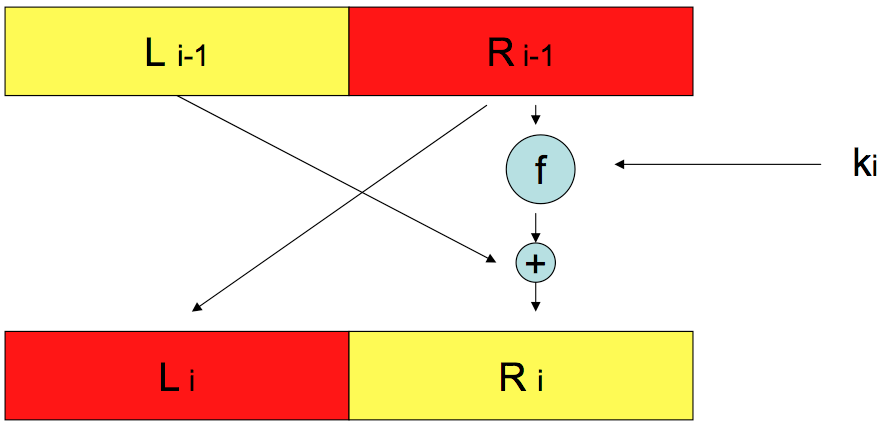
\includegraphics[scale=0.2]{horst-feistel.png} \\
\end{tabular}

\textbf{Die $f$-Funktion:} \\
\begin{center}
	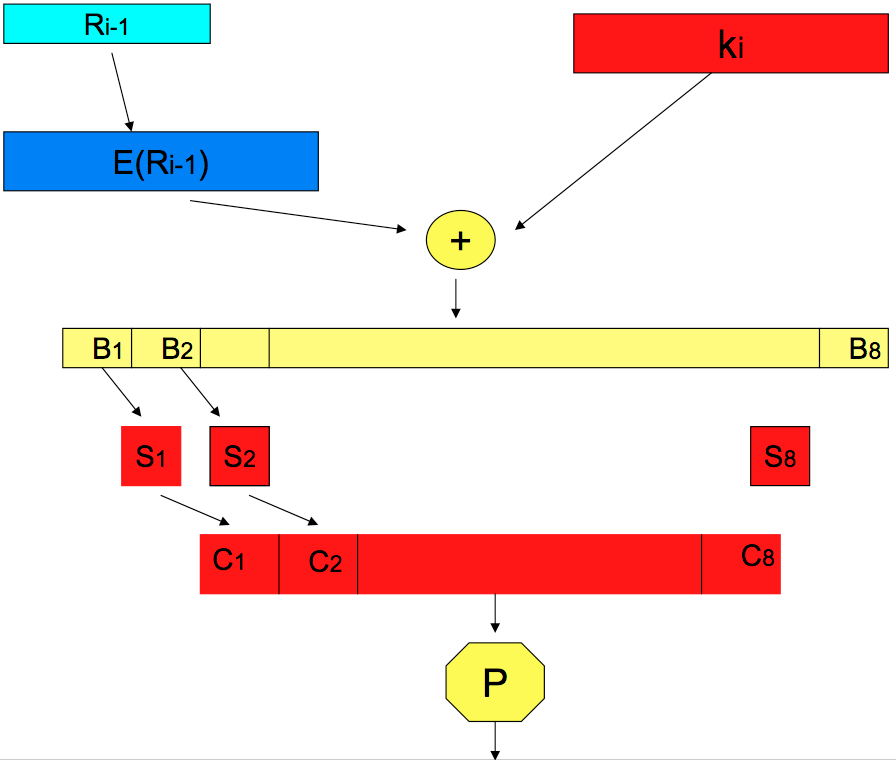
\includegraphics[scale=0.2]{funktion.png}
\end{center}
\subsection{Modi von Block-Cipher}
Sei $\Sigma:=\{0,1\}$\\ 
$p=c=\Sigma^4=\{\square\square\square\square\}$\\
$k=$ Permutation von $\Sigma^4$\\
$k=\pi=\Array{cccc}{1&2&3&4\\2&1&4&3}$\\
\subsubsection*{Vor- und Entschlüsselung}
Sei $m=0101\in p$ (Klartext)\\ 
$e_k(m)=e_k(0101)=1010=c$
\subsubsection{ECB-Modus (electronic code block)}
 $m=\underbrace{1100}_{m_1}|\underbrace{0110}_{m_2}|\underbrace{1100}_{m_3}|101^*$\\
 $\Unten{m_1}{\longrightarrow}$\fbox{$e_k$}$\Unten{c_1}{\longrightarrow}$\\
 \Bold{Bem:} \begin{enumerate}
              \item $m_1=m_3\Ra c_1=c_3$
              \item Vertauschen der Ciphertext-Blöcke wird nicht notwendigerweise erkannt
             \end{enumerate}
\subsubsection{CBC-Modus (cipher block chaining)}
\begin{tabular}{p{7.5cm}  l}
	$m=\Unten{\T{Länge n}}{m_1}|m_2|\dots$, $n:$ Blocklänge &\Bold{Bsp:} $m=\underbrace{1100}_{m_1} | \underbrace{0110}_{m_2} | \underbrace{1100}_{m_3} | 101$ \\
	{\color{red}IV = Initialvektor} (i.a. bekannt) &  $\color{red}IV=C_0=1110$  \\
	$C_0 := IV$ & $c_1 = e_k(c_0 \oplus m_1) = e_k(0010) = 0001$ \\
	$C_1 := e_k(C_0 \oplus m_1)$ & $c_2 = e_k(c_1 \oplus m_2) = e_k(0111) = 1011$ \\
	$C_2 := e_k(C_1 \oplus m_2)$  & $c_3 = e_k(c_2 \oplus m_3) = e_k(0111) = 1011$ \\
\end{tabular} \\ \\ \\
 \textbf{Entschlüsselung}: ${\color{red}c_1\oplus} d_k(c_2)={\color{red}c_1\oplus}d_k(e_k(c_1\oplus m_2))= c_1\oplus m_2 {\color{red}\oplus c_1 = m_2}$
 \begin{center}
	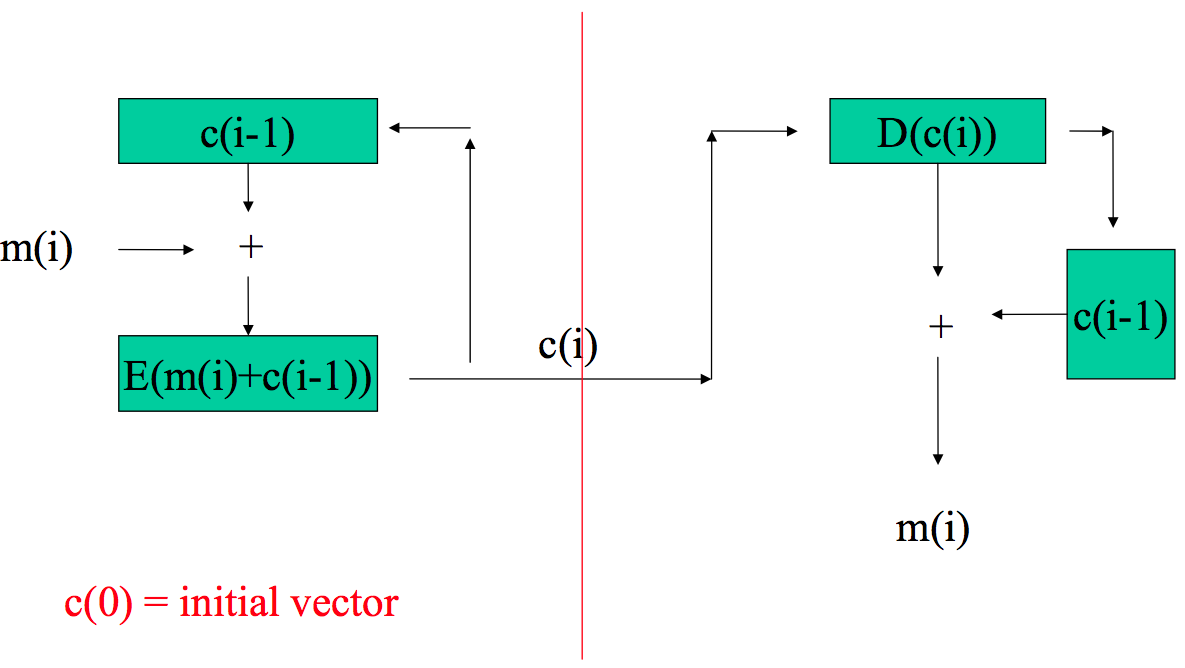
\includegraphics[scale=0.2]{cbc-encryption.png}
 \end{center}
 $m=\Unten{\T{Länge n}}{m_1}|m_2$, $n:$ Blocklänge\\
 $IV=$Initialvektor (i.a. bekannt)\\
 $c_0:=IV$, $c_1:=e_k(c_0\oplus m_1)$, $c_2:=e_k(c_1\oplus m_2)$\\
 $c_1\oplus d_k(c_2)=d_k(e_k(c_1\oplus m_2))=c_1\oplus m_2\oplus c_1=m_2$\\
 \Bold{Bsp:} $m=\underbrace{1100}_{m_1}|\underbrace{0110}_{m_2}|\underbrace{1100}_{m_3}|101$, $IV=c_0=1110$\\
 $c_1=e_k(c_0\oplus m_1)=e_k(0010)=0001$\\
 $c_2=e_k(c_1\oplus m_2)=e_k(0111)=1011$\\
 $c_3=e_k(c_2\oplus m_3)=e_k(0111)=1011$\\
 \Bold{Bem:} \begin{enumerate}
              \item $m_1=m_3\nRightarrow c_1=c_3$
              \item Vertauschen kann bemerkt werden
              \item Übertragungsfaktor machen sich bemerkbar
             \end{enumerate}
\subsubsection{CFB-Modus (cipher feedback)}
 $m=\underbrace{\tilde{m_1}}_{\T{Länge}=r}|\tilde{m_2}|\tilde{m_3}|\dots$, $n$: Cipher Block-Länge (DES: 64) und \fbox{$0<r\leq n$}\\
 \begin{tabular}{p{7.5cm}lr}
  \begin{tabular}{cl}
  $I_1$&$:=IV\in\Sigma^n$\\
  $\downarrow$\\
  \fbox{DES}\\
  $\downarrow$\\
  $O_1:\underbrace{\square}_{r}\square$\\
  $\oplus$&$\to c_1$\\
  $\tilde{m_1}\to\underbrace{\square}_{r}$\\
 \end{tabular}&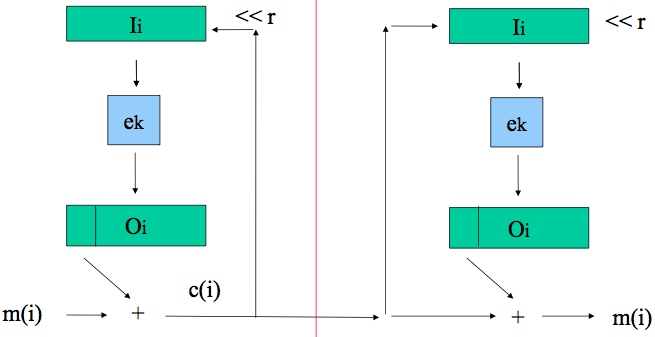
\includegraphics[scale=0.25]{cfb-encryption.png}\\
 \end{tabular}

 
 \Bold{Bsp:} $m=110|001|101|100|101$, $IV=1110$, \fbox{$r=3$, $n=4$}\\
 \begin{tabular}{cccccc}
  $I_1=$&$1110$&&$I_2=$&$\overbrace{111\mathbf{0}}^{I_1}\overbrace{\mathbf{000}}^{c_1}$\\
  &$\downarrow$&&&$\downarrow$\\
  &\fbox{$e_k$}&&&\fbox{$e_k$}\\
  &$\downarrow$&&&$\downarrow$\\
  $O_1$&$\mathbf{110}1$&&$O_2$&$\mathbf{000}0$\\
  &$\oplus$&$\to c_1=000$&&$\oplus$&$\to c_2=001$\\
  $\tilde{m_1}=$&$110$&&$\tilde{m_2}=$&$001$
 \end{tabular}
 
\newpage
\section{RSA}
\subsection{Schlüsselerzeugung}
PK = (n,e) \\
SK = (n,d) \\
Wir wählen zwei (grosse) Primzahlen p,q $\in \RN$*. $\varphi\neq q$ \\
$n=p*Q$ \\
$\varphi(n)=(p-1)(q-1)$ {\color{blue}// $\varphi(n) = |\ZN^*_n|$ }\\
{\color{blue}Wir wählen $e \in \ZN^*_{\varphi(n)}$} // ggT(e,$\varphi(n))=1$ \\
{\color{blue} $d:=e^{-1}$ in $\ZN^*_{\varphi(n)}$} // ed=1 in $\ZN^*_{\varphi(n)} \Leftrightarrow$ ed $\equiv$ 1 mod $\varphi(n)$\\ \\
$\Longrightarrow\varphi(n) | (ed-1)$\\ \\
$\Longrightarrow$ \fbox{$\exists k \in \ZN:e{\color{red}*d}+{\color{red}k*}\varphi(n))=1$} \\ \\
$d:=e^{-1}\in \ZN^*_{120}$ : \fbox{$ed+k\varphi(n)=1$} \\
\\
\textbf{Beispiel}: \\
$p=11$, $q=13$ \\
$n=p*q=143$ \\
$\varphi(n)=120=2^3*3*5$ \\
{\color{blue} e:=7} $\Rightarrow$ PK=(143,7) \\
$\ZN_n=\{0,1,2,3,\dots,n-1\}$ \\

\begin{tabular}{| c | c | c | c | c |}
	\hline
	i & $q_i$ & $r_i$ & $s_i$ & $t_i$ \\
	\hline
	0 & - & {\color{blue} 120} & {\color{red} 1} & {\color{red} 0} \\
	1 & {\color{red} 17} & {\color{blue} 7} & {\color{red} 0} & {\color{red} 1}\\
	\hline
	&&{\color{red} 1}&{\color{red} 1}&{\color{red} -17} \\
	\hline
\end{tabular} {\color{blue} 120=}{\color{red} q}$*${\color{blue} 7+}{\color{red} r} \\ \\
{\color{blue}$\Longrightarrow (*) \underbrace{e}_{7}*(-17)+1*\underbrace{\varphi(n)}_{120})=1$} {\color{red} // mod $\varphi(n) \Rightarrow$ \fbox{$d \equiv (-17)$ mod $\varphi(n)$}}

\subsection{Verschlüsselung und Entschlüsselung}
\subsubsection{RSA ist ein Blockcipher}

\begin{description}
	\item[encryption] : enc \\
		$\ZN_n \longrightarrow \ZN_n$ \\
		$m \longrightarrow c^e$ mod n
	\item[decyption] : dec \\
		$\ZN_n \longrightarrow \ZN_n$ \\
		$m \longrightarrow c^d$ mod n
\end{description} 
$\Brackar{l}{PK=(u,e) \\ SK=(u,d)}$ \fbox{$\forall m \in \ZN_n : dec_{\color{red}SK}((enc_{\color{red}PK}(m)))=m$} \\
\\
\subsubsection{Beweis}
\begin{description}
	\item[Fall 1:] \hfill \\
		ggT(m,n)=1 \\
		$(m^e)^d=m$ in $\ZN_n$ \\
		Weil ggT(m,n)=1 existiert das Inverse von m: $\underbrace{m^{ed-1}=1}_{\text{Das ist zu Zeigen!}}$ in $\ZN_n$ \\
		$e*d+k*\varphi(n)=1$ // Konstruktion des Schlüssel \\
		$\Rightarrow e*d-1=-k*\varphi(n) : m^{ed-1}=m^{-k*\varphi(n)}=(m^{-k})=1$ // Satz von Euler-Fermat  
	\item[Fall 2:] \hfill \\
		ggT(m,n)$\neq$1 $\Rightarrow m=l*p$ oder $m=k*q$ \\
\end{description}

\subsection{Hastad Attac}
\textbf{RSA} (n,e), (n,d) \\
\\
 \\
\begin{tabular}{l l l l l}
    & & {\color{red} $e=3$} & & $=x$ \\
	&  & Bob $(n_1,e)$ & : {\color{red}$c_1$} & $= m^3$ mod $n_1$\\
	&$\nearrow$  \\
	Alice & $\rightarrow$ & Jon $(n_2,e)$ & : {\color{red}$c_2$} & $= m^3$ mod $n_2$\\
	& $\searrow$ \\
	& & Paul $(n_3,e)$ & : {\color{red}$c_3$} & $= m^3$ mod $n_3$\\
\end{tabular}

$\underbrace{x}_{m^3} = c_1 y_1 M_1 + c_2 y_2 M_2 + c_3 y_3 M_3$ mod $n_1n_2n_3$ \\ 

\begin{tabular}{p{5cm}  p{5cm} l }
	$l=n_1n_2n_3$ & $y_iM_i\equiv 1$ mod $n_i$ & $y_i{\color{red}M_i} + \beta {\color{red}n_i}=1$\\
	$M_1 = \frac{l}{n_1} = n_2n_3$ \\
	$M_2 = \frac{l}{n_2} = n_1n_3$ \\
	$M_3 = \frac{l}{n_3} = n_1n_2$ \\
\end{tabular} \\ \\
\\
\begin{tabular}{p{5cm}  p{5cm} l }
	$m < min(n_1,n_2,n_3)$ & $x\equiv2$ mod $5$ & $crt([2,1,5],[5,7,9])$ \\
	& $x\equiv1$ mod $7$ \\
	$m*m*m < n_1n_2n_3$ & $x\equiv5$ mod $9$ & $y_1\equiv M_1.inverse\_mod(n_1)$ \\
\end{tabular} \\ \\
\\
\begin{tabular}{l l l}
	$\ZN_{n_1n_2n_3}$ & $\rightarrow$ & $\ZN_{n_1}$ x $\ZN_{n_2}$ x $\ZN_{n_3}$ \\
	x & $\rightarrow$ & (x mod $n1$,x mod $n_2$, x mod $n_3$) \\
	\\
	x & $\equiv$ 2 mod 5 & crt([2,1,5],[5,7,9]) \\
	x & $\equiv$ 1 mod 7 & $\rightarrow$ 302 \\
	x & $\equiv$ 5 mod 9 & $y_1 = M_1.inverse\_mod(n_1)$
\end{tabular}

\subsection{Bellare-Rogenwog plaintext-awarnes encription scheme}
\begin{description}
	\item[Def.] \hfill \\
		Ein Public-ky-Verschl. System heisst {\color{red} plaintext aware} \\
		$\Longleftrightarrow$ Es ist (praktisch) unmöglich einen {\color{red}gültigen} Ciphertext herzustellen, ohne den Plaintext zu kennen.
	\item[Gegeben] \hfill \\
		$f: \ZN^k_2 \longmapsto \ZN^k_2$ trapdoor Permutation (zb RSA) 
	\item[Bsp.] \hfill \\
		$k=1024$ $k_0=128$ $k_1=128$
\end{description}
$m=$Nachricht \\ 
$|m|\leq768$ \\ 
{\color{red} $r=$ random number} \\ \\
$\Brackar{l}{G: \ZN^{k_1}_2 \longrightarrow \ZN^{k-k_1}_2 \\ G: \ZN^{k-k_1}_2 \longrightarrow \ZN^{k_1}_2}$ "random" funktion
\begin{center}
\begin{tabular}{|c|c|c|}
\multicolumn{1}{c}{$k-k_0-k_1$}&\multicolumn{1}{c}{$k_0$}&\multicolumn{1}{c}{$k_1$}\\\hline
$m$ $\mid\mid$ padding & $0\dots\dots0$&{\color{red}$r$}\\\hline
\multicolumn{2}{c}{\raisebox{.5\normalbaselineskip}{$\underbrace{\hspace*{4cm}}$}}&\multicolumn{1}{c}{\raisebox{.5\normalbaselineskip}{$\underbrace{\hspace*{3cm}}$}}
\end{tabular}\\
 \begin{tikzpicture}
\tikzstyle{every node}=[draw,shape=circle];
\node (G) at (0,0) {$G$};
\node (plus) at (-2,0) {$+$};
\node (H) at (0,-2) {$H$};
\node (plus2) at (2,-2) {$+$};
\draw [->] (G) -- (plus);
\draw [->] (H) -- (plus2);
\draw [->] (-2,1) -- (plus);
\draw [->] (2,1) -- (plus2);
\draw [->] (2,0) -- (G);
\draw [->] (plus) -- (-2,-3);
\draw [->] (plus2) -- (2,-3);
\draw [->] (-2,-2) -- (H);
\end{tikzpicture}\\
\begin{tabular}{|c|c|}
\multicolumn{1}{c}{$\overbrace{\hspace*{4cm}}$}&\multicolumn{1}{c}{$\overbrace{\hspace*{5cm}}$}\\\hline
($m$ $\mid\mid$ padding $\mid 0\dots\dots0)\oplus G(r)$&$H((m\mid\mid$ padding $\mid 0\dots\dots0)\oplus G(r))\oplus r$\\\hline
\end{tabular}\\
\end{center}


\subsection{RSA-Probleme}
\subsubsection{Kleines $e$}
$p=next\_probable\_prime(2^{513}+\dots)$ \\
$q=next\_probable\_prime(2^{513}+\dots)$ \\
$n=p*q$ \\
$\phi=(p-1)*(q-1)$ \\
$e=3$ \\
$d=e.inverse\_mod(n)$ \\
${\color{red}PK =(n,e), SK=(n,e)}$ \\
$m=500000001230$ \\
$c=m.powermod(3,n)$\\
$cc=m^3$ \\
$c==cc$? \\
{\color{blue}
$\Rightarrow$ Alle Zahlen ($m$) die kleiner sind als $n$ werden nicht verschlüsselt. \\
$\Rightarrow$ Dies lässt sich mit einem grösseren $e$ lösen.
}

\newpage
\section{Keltenbrüche}
\begin{description}
	\item[Definition] \hfill \\
		Ein Ausdruck der From $a_0 + \frac{1}{a_1+\frac{1}{a_2+ \frac{1}{a_3+\frac{1}{a_n}}}}$ mit $a_0 \in \ZN$ \& $a_1,a_2,a_3$ \dots $\in \NN$* nennen wir endliche (reguläre) Keltenbrüche.
	\item[Notation] \hfill \\
		Wir schreiben dafür: $<a_0;a_1,a_2,a_2,$ \dots $,a_n>$
	\item[Entwicklung (KE)] \hfill \\
		Sei $a \in \QN \backslash \ZN$ // $\RN \backslash \ZN$ \\
		$\xi_0:=a$ \\
		$x_0:=[\xi_0]$ \\
		{\color{red}if} $\xi_0-x_0 \neq 0$ \\
		$\xi_1:=\frac{1}{\xi_0-x_0}$ \\
		$x_1:=[\xi_1]$ \\
		{\color{red}if} $\xi_1-x_1 \neq 0$ \\
		$\xi_2:=\frac{1}{\xi_1-x_1}$ \\
		$x_2:=[\xi_2]$
	\item[Beispiel] \hfill \\
		$\xi_0=\frac{37}{7}$ \\
		$x_0=[\xi_0]={\color{red}5}$ \\
		$\xi_1=\frac{1}{\xi_0-x_0}=\frac{1}{\frac{2}{7}}=\frac{7}{2}$ \\
		$x_1=[\xi_1]={\color{red}3}$ \\
		$\xi_2=\frac{1}{\xi_1-x_1}=\frac{1}{\frac{1}{2}}=2$ \\
		$x_2=[\xi_2]={\color{red}2}$ \\
		{\color{red} Ende} $\Rightarrow \frac{37}{7}=<5;3,2>$ \\
	\item[euklidischer Algorithmus] \hfill \\
		$\Brackar{l}{37={\color{red}5}*7+2 \\\\ 07={\color{red}3}*2+1 \\\\ 02={\color{red}2}*1}$
		\begin{tabular}{l}
			$\frac{37}{7}=5+\frac{2}{7}$ \\\\
			$\frac{7}{2}=3+\frac{1}{2}$ // $\frac{1}{\frac{7}{2}}=\frac{1}{3+\frac{1}{2}}$\\\\
			$\frac{2}{1}=2+\frac{0}{1}$ \\
		\end{tabular}  
	\item[Konvergente] \hfill \\
		Sei $a \in \QN \backslash \ZN (\RN \backslash \ZN)$ durch die KE gegeben: $a = <a_0;a_1,a_2,a_3,$ \dots, $a_n>$ \\
		Die Brüche: $<a_0>$, $<a_0;a_1>$, $<a_0;a_1,a_2>$,$<a_0;a_1,a_2,a_3>$, \dots, $<a_0;a_1,a_2,a_3,$\dots,$a_n>$ heissen die Konvergenten a.
	\item[Beispiel] \hfill \\
		$a=\frac{37}{7}$ \\
		Konvergenten: $5, 5+\frac{1}{3}=\frac{16}{3},\frac{37}{7}$ \\
		Sage: continued\_fraction\_list(37/7, partial\_convergents=True)
\end{description}

\newpage
\section{Uebungen}
\section*{Serie 4}
\subsection*{Aufgabe 1}
$m=$\begin{tabular}{|c|c|c|c|}\hline
 0011&0101&0110&0000\\\hline
\end{tabular}\\
\underline{Padding} 
\begin{tabular}{|c|c|c|c|c|c|c|c|}\hline
 1&1&1&1&0&0&0&0\\\hline
\end{tabular} $IV=c_0$ (bekannt)
\subsection*{Aufgabe 4 (Broadcast-attack)}
\Bold{Bem:} Sei $n=100$, $e=3$, $m\in\{0,1,2,3,4\}$, $m^e=(m^e$ mod $n)$\\
\Bold{Annahme:} 
\begin{tabular}{lll}
 &$\nearrow$&$c_1:=m^3$ mod $n_1$\\
 Alice&$\to$&$c_2:=m^3$ mod $n_2$\\
 $m$&$c_3:=m^3$ mod $n_3$
\end{tabular}\\
\Bold{$e=3$ für alle Teilnehmer}\\
$ggT(n_i,n_j)=1$, wenn $i\neq j$\\
$m<min(n_1,n_2,n_3)$

\section*{Serie 5}
\subsection*{Aufgabe 1}
$(n,e)$, $(n,d)$ RSA-Schlüssel Oscar\\
$(n,e_A)$, $(n,?)$ RSA-Schlüssel Alice\\
\Bold{unbekannt} $p,q$ $(n=p\cdot q)$ bzw. $\varphi(n)$\\
\Bold{Ziel:} Finde $\tilde{d_A}$ mit falls $c=m^{m_A}$ mod $n$ ist, gilt $m=c^{\tilde{d_A}}$ mod $n$\\
\Bold{Oscar:} $h:=e\cdot d-1$ (Es gilt $ed-k\varphi(n)=1$, $\varphi(n)\mid h$)\\
$h:=\frac{\Oben{k\varphi(n)}{h}}{ggT(\Unten{k\varphi(n)}{ed-1},e_A)}$ \hspace*{2cm}($ggT(e_A,\varphi(n))=1$, $\varphi(n)\mid h$)\\
$d:=ggT(h,e_A)$, $h:=\frac{h}{d}$ \hspace*{2cm}($\varphi(n)\mid h$)\\
$e_A\cdot\alpha+h\cdot\beta=1$\\
\fbox{$e_A\cdot\tilde{\alpha}+\varphi(n)\cdot\tilde{\beta}=1$} löst der Provider\\
$\tilde{d_A}:=\alpha$ mod $h$\\
\Bold{Behauptung:} $m = c^{\tilde{d_A}}$ mod $n=(m^{e_A})^{\tilde{d_A}}$ mod $n=m^{e_A\cdot \tilde{d_A}}$ mod $n=m^{1+h^{\tilde{\beta}}}=m\cdot (m^h)^{\tilde{\beta}}$ mod $n$ ($(m^h)^{\tilde{\beta}} = $
\begin{lstlisting}
 n = 78654787
 e = 11
 d = 64339331
 ea = 17
 c = m. power_mod(ea, n)
 h = e * d - 1
 gcd(h, ea) //1
 xgcd(ea, h) //1, alpha, beta
 dd = a % h
 mm = c. power_mod(dd, n)
 m = 1337
\end{lstlisting}


\end{document} 